\documentclass[12pt]{amsart}
\usepackage[margin=1in]{geometry}
\usepackage{amsmath,amssymb,enumitem,booktabs,tikz}
\newenvironment{solution}{\begin{proof}[Solution]}{\end{proof}}
\newcommand{\cart}{\mathbin{\square}}
\title{Exam2Prep}
\date{}
\begin{document}\maketitle

    \noindent Solutions to the exercises marked ($-$) in West, \emph{Introduction to Graph Theory}, second edition, Sections 3.1, 4.1, 4.2, and 5.1. The three optional exercises marked ($*-$) in Section 3.1 are included. Statements are condensed; qualifications needed for small or disconnected graphs are stated explicitly.

    \smallskip\noindent Notation: $n=n(G)$; $\alpha,\alpha',\beta,\beta'$ denote independence, matching, vertex-cover, and edge-cover numbers. $G+H$ is disjoint union, $G\vee H$ is join, and $G\cart H$ is Cartesian product. Connectivity means vertex connectivity unless specified otherwise.

    \section*{3.1 Matchings and Covers}

    \subsection*{3.1.1} Find a maximum matching and a minimum vertex cover in each of the three pictured bipartite graphs.
    \begin{solution}Label the top vertices $t_1,t_2,\ldots$ and the bottom vertices $b_1,b_2,\ldots$, each from left to right in the book. The following are explicit certificates:
        \begin{center}\begin{tabular}{ccl}\toprule
            Graph & Matching $M$ & Vertex cover $C$\\\midrule
            Left & $\{t_1b_3,t_3b_2,t_4b_5\}$ & $\{t_3,t_4,b_3\}$\\
            Middle & $\{t_1b_2,t_2b_3,t_4b_4\}$ & $\{t_4,b_2,b_3\}$\\
            Right & $\{t_1b_4,t_2b_1,t_3b_2,t_4b_5\}$ & $\{t_2,t_4,b_2,b_4\}$\\\bottomrule
            \end{tabular}\end{center}
        Each listed edge occurs in its graph, the matching edges have distinct endpoints, and the listed cover meets every edge. For any matching and vertex cover, $|M|\le |C|$, since distinct matching edges require distinct covering vertices. Equality therefore proves both optimality claims. The maximum matching sizes are $3,3,4$.\end{solution}

    \subsection*{3.1.2} Determine the minimum size of a maximal matching in $C_n$.
    \begin{solution}The answer is $\lceil n/3\rceil$ ($n\ge3$). If a maximal matching has $m$ edges, its $n-2m$ unmatched vertices must be independent. Between consecutive matching edges around the cycle there is at most one unmatched vertex, so $n-2m\le m$ and $m\ge\lceil n/3\rceil$.
    Conversely, put $m=\lceil n/3\rceil$. Around the cycle arrange $m$ disjoint matched pairs and $n-2m$ unmatched single vertices, placing at most one single between successive pairs. This is possible since $0\le n-2m\le m$. The unmatched vertices are independent, so the matching is maximal.\end{solution}

    \subsection*{3.1.3} If a matching saturates $S\subseteq V(G)$, prove that some maximum matching saturates $S$. Must every maximum matching do so?
    \begin{solution}Start with the given matching and repeatedly augment along an augmenting path until the matching is maximum. Augmentation preserves saturation of every previously saturated vertex: internal vertices exchange their matched edge, and the two endpoints become saturated. Thus the final matching saturates $S$.
    Not every maximum matching need do so. In $P_3=a b c$, take $S=\{a\}$. The maximum matching $\{ab\}$ saturates $S$, but the maximum matching $\{bc\}$ does not.\end{solution}

    \subsection*{3.1.4} Characterize the simple graphs for which each of $\alpha,\alpha',\beta,\beta'$ equals $1$.
    \begin{solution}\begin{itemize}[leftmargin=*]
\item $\alpha(G)=1$ exactly for nonempty complete graphs: every two distinct vertices must be adjacent.
\item $\alpha'(G)=1$ exactly for a nontrivial star or a triangle, together with any number of isolated vertices. To prove necessity, fix an edge $uv$. All edges meet $uv$. If all meet a single vertex, the nontrivial part is a star. Otherwise, if $u$ has two distinct neighbors $v,w$, an edge avoiding $u$ must be $vw$ (to meet both $uv$ and $uw$); any further edge would miss one of the three triangle edges. If the maximum degree is at most one, there is just one edge.
\item $\beta(G)=1$ exactly for a nontrivial star together with isolated vertices: one vertex meets every edge, and at least one edge exists.
\item $\beta'(G)=1$ exactly for $K_2$. One edge must cover every vertex, so there are exactly two vertices and they are adjacent. Graphs with isolated vertices have no edge cover.
        \end{itemize}\end{solution}

    \subsection*{3.1.5} Prove $\alpha(G)\ge n(G)/(\Delta(G)+1)$.
    \begin{solution}Greedily choose a remaining vertex for an independent set and delete its closed neighborhood. At most $\Delta(G)+1$ vertices are deleted at each step. The chosen vertices are independent, and if there are $s$ steps, then $n\le s(\Delta+1)$. Hence $\alpha(G)\ge s\ge n/(\Delta+1)$. As usual, graphs here are loopless.\end{solution}

    \subsection*{3.1.6} For a tree with $n$ vertices and independence number $k$, determine $\alpha'(T)$.
    \begin{solution}The complement of an independent set is a vertex cover, so $\beta(T)=n-\alpha(T)=n-k$. A tree is bipartite; the K\H{o}nig--Egerv\'ary theorem gives $\alpha'(T)=\beta(T)=n-k$.\end{solution}

    \subsection*{3.1.7} Prove that $G$ is bipartite iff $\alpha(H)=\beta'(H)$ for every subgraph $H$ without isolated vertices.
    \begin{solution}If $G$ is bipartite, so is $H$. The identities $\alpha(H)+\beta(H)=n(H)$ and $\alpha'(H)+\beta'(H)=n(H)$, together with $\alpha'(H)=\beta(H)$, give $\alpha(H)=\beta'(H)$ (the corollary cited in the exercise).
    Conversely, if $G$ is not bipartite, it contains an odd cycle $H=C_{2r+1}$. This subgraph has no isolated vertices, but $\alpha(H)=r$ and $\beta'(H)=r+1$: an edge cover needs at least $r+1$ edges and such a cover exists. Thus the stated equality fails.\end{solution}

    \subsection*{3.1.44} Suppose the degrees of any $k$ vertices sum to less than $n-k$. Prove every maximal independent set has more than $k$ vertices.
    \begin{solution}Assume $1\le k\le n$, and suppose an independent set $S$ has $s\le k$ vertices. Extend $S$ to a $k$-vertex set $R$. Degrees are nonnegative, so $\sum_{v\in S}d(v)\le\sum_{v\in R}d(v)<n-k$. Consequently
        \[
            \left|\bigcup_{v\in S}N[v]\right|\le s+\sum_{v\in S}d(v)<s+n-k\le n.
        \]
        Some vertex outside these closed neighborhoods can be added to $S$, so $S$ is not maximal.\end{solution}

    \subsection*{3.1.46 (optional)} Characterize graphs with domination number $1$.
    \begin{solution}Exactly the graphs with a universal vertex: $\gamma(G)=1$ iff some $v$ satisfies $N[v]=V(G)$, equivalently $d(v)=n-1$. This includes $K_1$.\end{solution}

    \subsection*{3.1.47 (optional)} Find a smallest tree whose domination and vertex-cover numbers differ.
    \begin{solution}Among nontrivial trees the minimum order is $6$, attained by $P_6=v_1\cdots v_6$. The set $\{v_2,v_5\}$ dominates it, and no vertex dominates all six vertices, so $\gamma(P_6)=2$. Its three disjoint edges $v_1v_2,v_3v_4,v_5v_6$ force $\beta(P_6)\ge3$, while $\{v_2,v_4,v_6\}$ is a cover, so $\beta(P_6)=3$.
    For minimality, every vertex cover of a graph without isolated vertices dominates it, so $\gamma\le\beta$. If a nontrivial tree has $\gamma=1$, it is a star and has $\beta=1$. Otherwise strict inequality requires $\beta\ge3$. Since a tree is bipartite, $\beta=\alpha'$, and three matching edges require at least six vertices.
        \emph{Convention:} if the one-vertex tree is allowed, $K_1$ is the trivial smaller exception, with $\gamma=1$ and $\beta=0$. The intended nontrivial-tree answer is $P_6$.\end{solution}

    \subsection*{3.1.48 (optional)} Determine $\gamma(C_n)$ and $\gamma(P_n)$.
    \begin{solution}Both equal $\lceil n/3\rceil$ (for $C_n$, $n\ge3$). Each vertex dominates at most three vertices, yielding the lower bound.
    For $P_n=v_1\cdots v_n$, if $n=3q$, choose $v_2,v_5,\ldots,v_{3q-1}$; if $n=3q+1$, add $v_{3q+1}$ to that set; if $n=3q+2$, add $v_{3q+2}$. These sets dominate the path and have the claimed size. Adding the edge $v_nv_1$ cannot destroy domination, so the same upper bound holds for the cycle.\end{solution}

    \section*{4.1 Cuts and Connectivity}

    \subsection*{4.1.1} Prove or refute the four assertions about vertex and edge connectivity.
    \begin{solution}\begin{enumerate}[label=(\alph*),leftmargin=*]
\item Every graph with connectivity $4$ is $2$-connected: true, since deleting fewer than two vertices leaves it connected.
\item Every $3$-connected graph has connectivity $3$: false. $K_5$ is $3$-connected but has connectivity $4$. The adjective $k$-connected means connectivity at least $k$.
\item Every $k$-connected graph is $k$-edge-connected: true, by $\kappa(G)\le\kappa'(G)$.
\item Every $k$-edge-connected graph is $k$-connected: false for $k=2$. Two triangles sharing exactly one vertex have no cut-edge, so they are $2$-edge-connected, but the shared vertex is a cut-vertex.
        \end{enumerate}\end{solution}

    \subsection*{4.1.2} Correct and prove: if $e$ is a cut-edge, then an endpoint of $e$ is a cut-vertex.
    \begin{solution}As stated this is false for $K_2$: its edge is a cut-edge, but neither vertex is a cut-vertex. Add the hypothesis that the component containing $e$ has at least three vertices (connected $G$ of order at least three suffices).
    Write $e=uv$, and let $A,B$ be the vertex sets of the two components obtained by deleting $e$ from its component, with $u\in A,v\in B$. At least one of $A,B$ has size at least two. If $|A|\ge2$, deletion of $u$ separates the nonempty sets $A-\{u\}$ and $B$, so $u$ is a cut-vertex. The case $|B|\ge2$ is symmetric.\end{solution}

    \subsection*{4.1.3} If an $n$-vertex simple graph other than $K_n$ is not $k$-connected, prove it has a separating set of size $k-1$.
    \begin{solution}Use the usual range $1\le k\le n-1$. There is a separating set $S$ with $|S|\le k-1$ (possibly empty for a disconnected graph). Choose $x,y$ in different components of $G-S$. Since $k-1\le n-2$, enlarge $S$ to a set $S'$ of size exactly $k-1$ while retaining $x,y$. No $x,y$-path exists in $G-S'$, since none exists in $G-S$. Thus $S'$ separates $G$.
    The upper restriction on $k$ is necessary; for $k=n$, deleting $n-1$ vertices leaves only one vertex and cannot disconnect the graph.\end{solution}

    \subsection*{4.1.4} Prove $G$ is $k$-connected iff $G\vee K_r$ is $(k+r)$-connected.
    \begin{solution}Assume the usual order requirement $n(G)>k$. If $G$ is $k$-connected, delete fewer than $k+r$ vertices from the join. If a vertex of $K_r$ remains, it is adjacent to every other remaining vertex, so the remaining graph is connected. If all $r$ new vertices are deleted, fewer than $k$ vertices of $G$ have been deleted, again leaving a connected graph.
    Conversely, if the join is $(k+r)$-connected, delete its $r$ new vertices and any set $S\subseteq V(G)$ with $|S|<k$. The total deletion has size less than $k+r$, so $G-S$ is connected. Hence $G$ is $k$-connected.\end{solution}

    \subsection*{4.1.5} Add all edges between vertices at distance $2$ in a connected graph $G$ of order at least $3$. Prove the resulting $G'$ is $2$-connected.
    \begin{solution}The graph $G'$ is connected. Fix a vertex $v$. Every component of $G-v$ has a neighbor of $v$, because $G$ is connected. Any two distinct neighbors of $v$ are adjacent in $G'$: their distance in $G$ is at most two. Thus, after deleting $v$, the components of $G-v$ are joined together in $G'-v$. Hence $G'-v$ is connected for every $v$, proving $2$-connectivity.\end{solution}

    \subsection*{4.1.6} For blocks $B_1,\ldots,B_b$, prove the vertex-count identity $n(G)=\sum_i n(B_i)-b+1$.
    \begin{solution}This identity needs $G$ to be connected. For a connected graph, induct on the number of blocks. The one-block case is immediate. An end-block $B$ meets the remaining connected graph $H$ in exactly one cut-vertex, so $n(G)=n(H)+n(B)-1$. Applying induction to $H$ gives the formula.
    For a graph with $c$ components, summing the connected formulas gives the corrected general identity
        \[
            n(G)=\sum_{i=1}^{b}n(B_i)-b+c,
        \]
        counting each isolated vertex as a block. For example, $2K_2$ disproves the printed formula without connectedness.\end{solution}

    \subsection*{4.1.7} Express the number of spanning trees of a connected graph in terms of its blocks.
    \begin{solution}Writing $\tau(H)$ for the number of spanning trees,
        \[
            \tau(G)=\prod_{i=1}^{b}\tau(B_i).
        \]
        Choose a spanning tree independently in each block. Their union is connected because the blocks connect through cut-vertices, and acyclic because every cycle of $G$ is contained in one block. Conversely, a spanning tree restricts to a spanning tree of each block: a path cannot leave a block and reenter through another vertex, since that would combine blocks into a larger subgraph without a cut-vertex. These operations are inverse, giving the product. Bridge blocks and isolated-vertex blocks contribute a factor of one.\end{solution}

    \subsection*{4.1.30} On $\{1,\ldots,11\}$, join distinct integers with a common factor greater than $1$. Determine the blocks.
    \begin{solution}The even vertices $\{2,4,6,8,10\}$ induce $K_5$, and $\{3,6,9\}$ induces a triangle. These two cliques share only vertex $6$. Vertex $5$ has only neighbor $10$, while $1,7,11$ are isolated. The complete block list is therefore
        \[
            G[\{2,4,6,8,10\}]\cong K_5,\quad
            G[\{3,6,9\}]\cong K_3,\quad
            G[\{5,10\}]\cong K_2,
        \]
        together with the three isolated-vertex blocks. The cut-vertices are $6$ and $10$; the only edge between $5$ and the rest is $5\,10$.\end{solution}

    \section*{$4.2$ $k$-Connected Graphs}

    \subsection*{4.2.1} Determine $\kappa(u,v)$ and $\kappa'(u,v)$ in the pictured graph, with optimality certificates.
    \begin{solution}Label the three vertices in the middle vertical column $a,b,c$ from top to bottom, and the vertex immediately right of $b$ by $d$. Label the four vertices one column right of $u$ by $p,q,r,s$ from top to bottom, and those one column left of $v$ by $P,Q,R,S$ from top to bottom. Parallel edges in the drawing are distinct.
    Three internally disjoint paths are
        \[
            u p a P v,\qquad u q b d Q v,\qquad u s c S v.
        \]
        Deleting $\{a,b,c\}$ separates $u$ from $v$. Thus $\kappa(u,v)=3$.
        Five edge-disjoint paths are
        \[
            u p a P v,\quad u q a Q v,\quad u q b d Q v,
            \quad u r c R v,\quad u s c S v.
        \]
        The two occurrences of $uq$ use its two parallel edges, and the two occurrences of $Qv$ use its two parallel edges. The five edges
        \[
            pa,\ qa,\ bd,\ rc,\ sc
        \]
        separate $\{u,p,q,r,s,b\}$ from all remaining vertices. Thus $\kappa'(u,v)=5$. Each lower bound comes from disjoint paths; each matching upper bound comes from a cut.\end{solution}

    \subsection*{4.2.2} Prove subdivision preserves $2$-edge-connectivity, and deduce that a graph with a closed-ear decomposition is $2$-edge-connected.
    \begin{solution}A connected graph is $2$-edge-connected iff every edge lies on a cycle. Subdividing $xy$ into $xw,wy$ preserves connectedness. Replace $xy$ by $xwy$ in any cycle using $xy$; hence each new edge lies on a cycle, and every old edge still does.
    For the deduction, start with the initial cycle. An open ear can be formed by adding an edge between its old endpoints and subdividing it; the new edge lies on a cycle using an old path. A closed ear can be formed by adding a new vertex with two parallel edges to its old endpoint, then subdividing those edges. These operations preserve connectedness and put every edge on a cycle. Induction over the ears proves the result.\end{solution}

    \subsection*{4.2.3} In the divisibility digraph on $[12]$, determine $\kappa(1,12)$ and $\kappa'(1,12)$.
    \begin{solution}The arc $1\to12$ exists. Therefore no deletion of vertices other than $1,12$ can destroy reachability from $1$ to $12$: the vertex-cut parameter $\kappa(1,12)$ is undefined under the book's convention for adjacent ordered pairs (or infinite if an extended minimum convention is adopted).
    There are five edge-disjoint directed paths
        \[
            1\to12,\qquad 1\to j\to12\quad(j=2,3,4,6).
        \]
        The only arcs entering $12$ from other vertices come from $1,2,3,4,6$. Deleting these five arcs blocks every path, proving $\kappa'(1,12)=5$. Loops, if included in the divisibility relation, affect neither conclusion.\end{solution}

    \subsection*{4.2.4} Must every given $u,v$-path in a $2$-connected graph have an internally disjoint $u,v$-path?
    \begin{solution}No. Take $G=K_4-uv$, with vertices $u,v,x,y$, and let $P=u x y v$. The cycle $u x v y u$ spans $G$, so $G$ is $2$-connected. An internally disjoint path from $u$ to $v$ would have to avoid both $x$ and $y$, requiring the missing edge $uv$. Menger's theorem guarantees some pair of internally disjoint paths, not a partner for every prescribed path.\end{solution}

    \subsection*{4.2.5} Join $u,v$ in $H(G)$ iff they occur on a common cycle of the simple graph $G$. Characterize when $H(G)$ is complete.
    \begin{solution}For $n(G)\ge3$, exactly when $G$ is $2$-connected. If $G$ is $2$-connected, two internally disjoint paths between any two vertices form a cycle through them, so $H(G)$ is complete. Conversely, completeness implies that every pair is on a cycle, so $G$ is connected. If $x$ were a cut-vertex, vertices in distinct components of $G-x$ could not lie on a common cycle: deleting $x$ from such a cycle would leave a path joining those components. Thus $G$ has no cut-vertex.
    For completeness about small orders: $G=K_1$ gives the vacuous exception $H(G)=K_1$; no two-vertex simple graph satisfies the condition.\end{solution}

    \subsection*{4.2.6} Prove that a simple graph is $2$-connected iff it is obtainable from $C_3$ by edge additions and subdivisions.
    \begin{solution}Edge addition preserves $2$-connectivity. Subdivision also does: if $xy$ becomes $xw,wy$, deleting $w$ leaves $G-xy$, which is connected since no edge of a $2$-connected graph is a bridge. Deleting an old vertex leaves a connected graph, with $w$ either on a subdivided old edge or attached to the surviving endpoint of $xy$.
    For necessity, take an open-ear decomposition of $G$. Obtain its initial cycle by subdividing edges of $C_3$. To add an ear with old endpoints $x,y$, if $xy$ is absent, add $xy$ and subdivide it to the ear's length. If $xy$ is already present, subdivide that existing edge to form the new ear and then add $xy$ back. In the latter case the ear has length at least two, so all intermediate graphs can remain simple. These operations realize every ear addition.\end{solution}

    \section*{5.1 Vertex Coloring and Upper Bounds}

    \subsection*{5.1.1} Compute the clique, independence, and chromatic numbers of the pictured graph. Check the standard lower bounds and color-criticality.
    \begin{solution}\begin{center}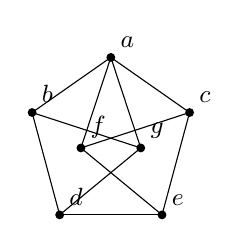
\begin{tikzpicture}[scale=1,every node/.style={font=\small}]
                                      \coordinate (a) at (0,2);
                                      \coordinate (b) at (-1,1.3);
                                      \coordinate (c) at (1,1.3);
                                      \coordinate (d) at (-0.65,0);
                                      \coordinate (e) at (0.65,0);
                                      \coordinate (f) at (-0.38,0.85);
                                      \coordinate (g) at (0.38,0.85);
                                      \draw (a)--(b);
                                      \draw (a)--(c);
                                      \draw (a)--(f);
                                      \draw (a)--(g);
                                      \draw (b)--(d);
                                      \draw (b)--(g);
                                      \draw (c)--(e);
                                      \draw (c)--(f);
                                      \draw (d)--(e);
                                      \draw (e)--(f);
                                      \draw (d)--(g);
                                      \fill (a) circle (1.6pt) node[above right] {$ a $};
                                      \fill (b) circle (1.6pt) node[above right] {$ b $};
                                      \fill (c) circle (1.6pt) node[above right] {$ c $};
                                      \fill (d) circle (1.6pt) node[above right] {$ d $};
                                      \fill (e) circle (1.6pt) node[above right] {$ e $};
                                      \fill (f) circle (1.6pt) node[above right] {$ f $};
                                      \fill (g) circle (1.6pt) node[above right] {$ g $};
        \end{tikzpicture}\end{center}
        Use the labels above. The triangles are $abg$ and $acf$, so $\omega(G)=3$; neither extends to a $4$-clique. Also $\alpha(G)=2$: $\{b,c\}$ is independent, and for every vertex its nonneighbors induce a clique (check from the displayed edges), ruling out an independent triple. Hence
        \[
            \chi(G)\ge\left\lceil\frac{7}{2}\right\rceil=4.
        \]
        A proper $4$-coloring in the order $(a,b,c,d,e,f,g)$ is $(1,2,2,1,3,4,3)$. Thus $\chi(G)=4$. The independence bound proves optimality; the clique bound $\chi\ge3$ does not.
        The graph is color-critical, even under edge deletion. Here are proper $3$-colorings after deleting each edge; each tuple is ordered $(a,b,c,d,e,f,g)$.
        \begin{center}\begin{tabular}{cc}\toprule Deleted edge & Color tuple\\\midrule
            $ab$ & $1,1,2,2,1,3,3$\\
            $ac$ & $1,2,1,1,2,3,3$\\
            $af$ & $1,2,2,1,3,1,3$\\
            $ag$ & $1,2,2,3,1,3,1$\\
            $bd$ & $1,2,2,2,1,3,3$\\
            $bg$ & $1,2,2,3,1,3,2$\\
            $ce$ & $1,2,2,1,2,3,3$\\
            $cf$ & $1,2,2,1,3,2,3$\\
            $de$ & $1,2,2,1,1,3,3$\\
            $ef$ & $1,2,2,1,3,3,3$\\
            $dg$ & $1,2,2,3,1,3,3$\\
            \bottomrule\end{tabular}\end{center}
        Every proper subgraph omits an edge or vertex; since the graph has no isolated vertices, it is a subgraph of some $G-e$. Therefore every proper subgraph is $3$-colorable.\end{solution}

    \subsection*{5.1.2} Prove $\chi(G)$ is the maximum chromatic number of its components.
    \begin{solution}Every coloring of $G$ restricts to a coloring of every component, giving the lower bound. For the upper bound, color each component using the same palette of $r=\max_C\chi(C)$ colors. There are no edges between components, so their colorings combine to a proper $r$-coloring.\end{solution}

    \subsection*{5.1.3} Prove $\chi(G)=\max_i\chi(B_i)$ for the blocks $B_i$ of $G$.
    \begin{solution}Each block is a subgraph, giving $\chi(G)\ge\max_i\chi(B_i)$. Within a connected component, inductively attach end-blocks, using $r=\max_i\chi(B_i)$ colors in every block. An attached block meets the previously colored graph in one cut-vertex; permute its color names so the two colorings agree there. No other compatibility is needed. This colors each component with $r$ colors, and the same palette works across components.\end{solution}

    \subsection*{5.1.4} Exhibit $G,v$ with $\chi(G-v)<\chi(G)$ and $\chi(\overline G-v)<\chi(\overline G)$.
    \begin{solution}Take $G=C_5$ and any vertex $v$. Both $G$ and $\overline G\cong C_5$ have chromatic number $3$. Deleting a vertex from either yields $P_4$, of chromatic number $2$.\end{solution}

    \subsection*{5.1.5} Prove $\chi(G+H)=\max\{\chi(G),\chi(H)\}$ and $\chi(G\vee H)=\chi(G)+\chi(H)$.
    \begin{solution}For disjoint union, the component argument allows the same palette on both graphs, while restriction gives the lower bound. In a join, every vertex of $G$ is adjacent to every vertex of $H$, so the two graphs must use disjoint palettes. They need at least $\chi(G)+\chi(H)$ colors, and optimal colorings with disjoint palettes attain that number.\end{solution}

    \subsection*{5.1.6} If $\chi(G)=\omega(G)+1$, put $H_1=G$ and $H_k=H_{k-1}\vee G$. Prove $\chi(H_k)=\omega(H_k)+k$.
    \begin{solution}The join of $k$ copies of $G$ has $\chi(H_k)=k\chi(G)$ by Exercise 5.1.5. A clique in a join consists of a clique from each factor, so $\omega(H_k)=k\omega(G)$. Therefore $\chi(H_k)=k(\omega(G)+1)=\omega(H_k)+k$.\end{solution}

    \subsection*{5.1.7} Give a graph, neither a clique nor an odd cycle, and an order for which greedy coloring uses $\Delta(G)+1$ colors.
    \begin{solution}Take the path $v_1v_2v_3v_4$, and order its vertices as $v_1,v_4,v_2,v_3$. First-fit greedy coloring gives colors $1,1,2,3$ in that order. Thus it uses $3=\Delta(P_4)+1$ colors, although the path is $2$-colorable.\end{solution}

    \subsection*{5.1.8} Prove $\max_{H\subseteq G}\delta(H)\le\Delta(G)$, and characterize equality.
    \begin{solution}For every nonempty subgraph $H$, $\delta(H)\le\Delta(H)\le\Delta(G)$, proving the inequality and showing that the degeneracy bound on $\chi(G)$ is at least as strong as the maximum-degree bound.
    Let $D=\Delta(G)$. If some $H$ has $\delta(H)=D$, then every vertex of $H$ has degree exactly $D$ in both $H$ and $G$. Thus no edge incident to a vertex of $H$ is omitted, and no such vertex has a neighbor outside $H$. Therefore $H$ is a union of $D$-regular components of $G$. Conversely, a $D$-regular component has minimum degree $D$. Equality holds exactly when $G$ has a $\Delta(G)$-regular component.\end{solution}

    \subsection*{5.1.9} Draw and optimally color $K_{1,3}\cart P_3$; give a $3$-coloring of $C_5\cart C_5$ with class sizes $9,8,8$.
    \begin{solution}Let $x$ be the star center, its leaves $a,b,c$, and $j=0,1,2$ the path coordinate. Draw three copies of the star and join corresponding vertices of successive copies:
        \begin{center}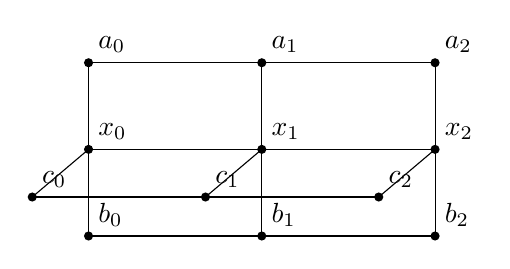
\begin{tikzpicture}[scale=1.1]
                          \foreach \j in {0,1,2}{
                              \coordinate (x\j) at (2*\j,0);
                              \coordinate (a\j) at (2*\j,1);
                              \coordinate (b\j) at (2*\j,-1);
                              \coordinate (c\j) at (2*\j-.65,-.55);
                              \foreach \v in {a,b,c}{\draw (x\j)--(\v\j);}
                              \foreach \v in {x,a,b,c}{\fill (\v\j) circle (1.5pt) node[above right] {$\v_{\j}$};}
                          }
                          \foreach \v in {x,a,b,c}{\draw (\v0)--(\v1)--(\v2);}
            \end{tikzpicture}\end{center}
        Set $s(x)=0$ and $s(a)=s(b)=s(c)=1$. The coloring $s(v)+j\pmod2$ is proper: every edge changes exactly one parity. Since the graph has edges, $\chi=2$.
        For $C_5\cart C_5$, use the grid below with both row and column indices taken cyclically. Join consecutive entries in each row and column, including the wraparound pairs; this is the toroidal drawing of the product.
        \[
            \begin{array}{c|ccccc}
                &0&1&2&3&4\\\hline
                0&1&2&0&1&2\\
                1&2&0&1&2&0\\
                2&0&1&2&0&1\\
                3&1&2&0&1&2\\
                4&2&0&1&2&0
            \end{array}
        \]
        Consecutive entries, including wraparound entries, differ in every row and column. Color $2$ occurs nine times; colors $0,1$ occur eight times each. A row is a $5$-cycle, so three colors are also optimal.\end{solution}

    \subsection*{5.1.10} Prove $G\cart H$ decomposes into $n(G)$ copies of $H$ and $n(H)$ copies of $G$.
    \begin{solution}For each $g\in V(G)$, the vertices $(g,h)$ induce a copy of $H$ using exactly the edges whose first coordinates agree. For each $h\in V(H)$, the vertices $(g,h)$ induce a copy of $G$ using exactly the edges whose second coordinates agree. Every product edge has exactly one of these two types, so the copies partition the edge set. Copies of different types may share vertices; a decomposition requires disjoint edge sets.\end{solution}

    \subsection*{5.1.11} Prove each of the two pictured graphs is isomorphic to $C_3\cart C_3$.
    \begin{solution}Use coordinates $(i,j)\in\{1,2,3\}^2$. In the left drawing, label the six outer vertices clockwise starting at the top by
        \[
            (1,1),(2,1),(2,3),(3,3),(3,2),(1,2),
        \]
        and label the inner vertices (top, lower-left, lower-right) by
        \[
            (2,2),(1,3),(3,1).
        \]
        In the right drawing, label the nine perimeter vertices clockwise starting at the top by
        \[
            \begin{gathered}
                (1,1),(1,2),(1,3),(2,3),(2,1),\\
            (2,2),(3,2),(3,3),(3,1).
            \end{gathered}
        \]
        In each drawing, inspection of its edges gives the six triangles obtained by fixing either coordinate. Every vertex has degree four, with its neighbors precisely the other two vertices in its row and the other two in its column. Thus two vertices are adjacent exactly when their coordinate pairs agree in one coordinate and differ in the other, which is the adjacency rule for $C_3\cart C_3$. These bijections are the required isomorphisms.\end{solution}

    \subsection*{5.1.12} Must a $k$-chromatic graph have a proper $k$-coloring with a color class of size $\alpha(G)$?
    \begin{solution}No. Join the centers $u,v$ of two disjoint copies of $K_{1,2}$. This six-vertex tree has two leaves at each center. Its four leaves form a maximum independent set: choosing either center excludes its two leaves and the other center, leaving an independent set of size at most three. Thus $\alpha(G)=4$.
    The graph is connected and bipartite, so its bipartition is unique up to swapping. Each part consists of one center and the two leaves at the other center, and has size three. Every proper $2$-coloring therefore has classes of size $3,3$, never four.\end{solution}

    \subsection*{5.1.13} If $G=F\cup H$, must $\chi(G)\le\chi(F)+\chi(H)$?
    \begin{solution}No. On the same six vertices split into two triples, take $F=K_{3,3}$ and let $H$ consist of the two triangles within the triples. Then $F\cup H=K_6$, but $\chi(F)=2$, $\chi(H)=3$, and $\chi(K_6)=6>5$.\end{solution}

    \subsection*{5.1.14} Prove or refute $\chi(G)\le n(G)-\alpha(G)+1$.
    \begin{solution}True. Give one color to a maximum independent set, and give a distinct new color to each remaining vertex. This uses $1+n(G)-\alpha(G)$ colors and is proper.\end{solution}

    \subsection*{5.1.15} For connected $G$, must $\chi(G)\le1+a(G)$, where $a(G)$ is the average degree?
    \begin{solution}No. Start with $K_4$ and attach a path of three new vertices to one clique vertex, using three new edges. The resulting graph has $n=7$, $e=9$, average degree $a=18/7$, and chromatic number $4$ (the clique requires four colors, which extend along the path). But $1+a=25/7<4$.\end{solution}

    \subsection*{5.1.16} Use Theorem 5.1.21 to prove every tournament has a spanning directed path.
    \begin{solution}An $n$-vertex tournament is an orientation of $K_n$, and $\chi(K_n)=n$. The Gallai--Roy theorem gives a directed path of length at least $\chi(K_n)-1=n-1$. A path has distinct vertices, so this path contains all $n$ vertices. The one-vertex case is immediate.\end{solution}

    \subsection*{5.1.17} Use Lemma 5.1.18 to prove $\chi(G)\le4$ for the pictured six-vertex graph.
    \begin{solution}Label the outer pentagon $a,b,c,d,e$ clockwise from the top and its central vertex $f$. The edges are the pentagon edges and $fb,fc,fd,fe$. The degrees are $2,3,3,3,3,4$, respectively. If $\chi(G)\ge5$, then $G$ contains a $5$-critical subgraph, whose minimum degree is at least four by the lemma. But only $f$ can even have degree four in a subgraph of $G$, so no such subgraph exists. Hence $\chi(G)\le4$.
    In fact $\chi(G)=3$: the color classes $\{a,f\}$, $\{b,d\}$, $\{c,e\}$ are independent, and $b,c,f$ form a triangle.\end{solution}

    \subsection*{5.1.18} How many colors are needed on $V(K_n)$ if every color class must induce maximum degree at most $k$?
    \begin{solution}For $k\ge0$, the answer is $\lceil n/(k+1)\rceil$. A color class of size $s$ induces $K_s$, whose maximum degree is $s-1$. Thus each class has at most $k+1$ vertices, forcing the lower bound. Partitioning the vertices into groups of size at most $k+1$ attains it. This is a relaxed coloring, not necessarily a proper coloring when $k>0$.\end{solution}

    \subsection*{5.1.19} Find the error in the proposed inductive proof of Brooks\textquotesingle\ theorem that colors pieces separated by $S$ and permutes colors to agree on $S$.
    \begin{solution}The claimed compatibility on $S$ is unjustified. A permutation of color names preserves which vertices have equal colors. If nonadjacent vertices $x,y\in S$ have the same color in one piece and different colors in another, no permutation makes both restrictions agree. An arbitrary separating set need not be a clique, so its coloring need not have a unique equality pattern. The separate colorings therefore cannot simply be glued as asserted.\end{solution}

    \subsection*{5.1.49} $2$-color the Petersen graph so each color class induces only isolated edges and vertices.
    \begin{solution}Use the standard representation with outer vertices $u_i$, inner vertices $v_i$ ($i\in\mathbb Z_5$), outer edges $u_iu_{i+1}$, inner edges $v_iv_{i+2}$, and spokes $u_iv_i$. Assign the colors in the following table:
        \begin{center}\begin{tabular}{c|ccccc}
                          $i$&0&1&2&3&4\\\hline
                          $u_i$&R&R&B&R&B\\
                          $v_i$&B&B&R&R&R\\
            \end{tabular}\end{center}
        The only monochromatic edges are $u_0u_1,\ v_2v_4,\ u_3v_3$. They have pairwise disjoint endpoints. Thus both induced color-class subgraphs have maximum degree at most one, so each consists of isolated edges and isolated vertices.\end{solution}

    \clearpage
    \section*{Homework 5 --- Book Section 3.1}

    \subsection*{Homework 5, Problem 1} let $S$ be the set of vertices saturated by a matching $M$ in a graph $G$.
    Prove that some maximum matching also saturates all of $S$.
    (Hint: Use Berge's Theorem to show that on can start with any matching $M$, and find a sequence of
    ``alternating path augmentations'' that produce a maximum matching $M^*$.
    Be careful not to conflate ``maximum'' with ``maximal.'')

    \begin{solution}
        Start with $M_0=M$. If $M_i$ is not maximum, Berge's Theorem
        gives an $M_i$-augmenting path $P$: its edges alternate between
        edges outside and inside $M_i$, and its two endpoints are
        unsaturated by $M_i$. Set
        \[
            M_{i+1}=M_i\mathbin{\triangle}E(P).
        \]
        This is a matching with $|M_{i+1}|=|M_i|+1$. Every internal
        vertex of $P$ loses one matching edge and gains one, the two
        endpoints become saturated, and vertices outside $P$ retain
        their matching status. Thus every vertex saturated by $M_i$
        is also saturated by $M_{i+1}$.

        Since a matching has at most $\lfloor |V(G)|/2\rfloor$ edges,
        this process terminates. At termination there is no augmenting
        path, so Berge's Theorem implies that the resulting matching
        $M^*$ is maximum. Saturation is preserved at every step; hence
        $M^*$ saturates all of $S$.
    \end{solution}

    \subsection*{Homework 5, Problem 2} Determine the minimum size of a maximal matching in the cycle $C_n$,

    \begin{solution}
        For every $n\geq 3$, the minimum size is
        \[
            \left\lceil\frac{n}{3}\right\rceil.
        \]
        A matching is maximal precisely when no edge has two
        unsaturated endpoints: such an edge could be added, and any
        edge that could be added would have two unsaturated endpoints.
        Consequently, every edge of $C_n$ either belongs to a maximal
        matching $M$ or shares an endpoint with an edge of $M$.
        Each matching edge accounts for at most three cycle edges
        (itself and its two neighboring edges). Therefore
        $n\leq 3|M|$, giving the lower bound
        $|M|\geq\lceil n/3\rceil$.

        For a construction attaining this bound, label the vertices
        $v_1,\ldots,v_n$ in cyclic order, write $n=3q+r$ with
        $r\in\{0,1,2\}$, and start with
        \[
            M_0=\{v_{3j+1}v_{3j+2}:0\leq j\leq q-1\}.
        \]
        If $r=0$, take $M=M_0$. If $r=1$, take
        $M=M_0\cup\{v_{3q}v_{3q+1}\}$. If $r=2$, take
        $M=M_0\cup\{v_{3q+1}v_{3q+2}\}$.
        In every case these edges are pairwise disjoint and the
        unsaturated vertices are pairwise nonadjacent, including
        across the edge $v_nv_1$. Thus $M$ is maximal. Its size is
        $q$ when $r=0$ and $q+1$ otherwise, as required.
    \end{solution}

    \subsection*{Homework 5, Problem 3} Let $M$ and $M'$ be matchings in an $X,Y$-bigraph $G$.
    Suppsose that $M$ saturates $S\subseteq X$ and $M'$ saturates $T\subseteq Y$.
    Prove that $G$ has a matching that saturates $S \cup T$

    \begin{solution}
        Consider the spanning subgraph $H$ with edge set $M\cup M'$.
        Every vertex has degree at most two. Each edge in $M\cap M'$
        is an isolated edge component. Every other nontrivial
        component is a path or an even cycle whose edges alternate
        between $M$ and $M'$.

        On a cycle, either set of alternating edges saturates every
        vertex. On an isolated common edge, choose that edge. On a
        path component, every internal vertex is saturated by both
        matchings, so only its endpoints can require a choice.
        An endpoint in $S$ can require the $M$-edges, and an endpoint
        in $T$ can require the $M'$-edges.

        These requirements cannot conflict on a single path.
        Indeed, a conflict would give an endpoint $s\in S\subseteq X$
        incident only with an $M$-edge and another endpoint
        $t\in T\subseteq Y$ incident only with an $M'$-edge.
        The alternating path from $s$ to $t$ would then have even
        length, since its first and last edges belong to different
        matchings. An even-length path in a bipartite graph has its
        endpoints in the same part, contradicting $s\in X$ and
        $t\in Y$.

        On each path choose the set of alternating edges satisfying
        its endpoint requirements, choosing either set if there are
        none. Isolated vertices belong to neither $S$ nor $T$.
        The union of all chosen edges is a matching, since distinct
        components are vertex-disjoint, and it saturates $S\cup T$.
    \end{solution}

    \subsection*{Homework 5, Problem 4} When $k\ge 2$, prove that $Q_k$ has at least $2^{2^{k-2}}$ perfect matchings

    \begin{solution}
        Represent the vertices of $Q_k$ by binary strings of length
        $k$, with two vertices adjacent when they differ in exactly
        one coordinate. Fixing the last $k-2$ coordinates and varying
        the first two gives a copy of $Q_2$, that is, a $4$-cycle.
        The $2^{k-2}$ possible fixed strings partition $V(Q_k)$ into
        $2^{k-2}$ vertex-disjoint $4$-cycles.

        Each of these cycles has two perfect matchings. Choose one
        independently in each cycle and take their union. The union
        is a perfect matching of $Q_k$, since it saturates every
        vertex exactly once. Different choices give different
        perfect matchings: a change on any one cycle changes the
        edges of the union. Hence $Q_k$ has at least
        \[
            2^{\,2^{k-2}}
        \]
        perfect matchings. This also covers $k=2$, when the fixed
        string is empty and there is a single $4$-cycle.
    \end{solution}

    \subsection*{Homework 5, Problem 5} Let $G$ be the Petersen Graph.
    \begin{itemize}
        \item[(a)] Prove that deleting any perfect matching of $G$ leaves $C_5 + C_5$ (i.e. two disjoint 5-cycles).
        (Hint: After you remove a perfect matching what is the degree of each vertex).
        \item[(b)] Prove that the Petersen graph has exactly six perfect matchings.
        (Hint: use (a) and use the fact that you already know how many 5-cycles $G$ contains.)
    \end{itemize}

    \begin{solution}
        Use the standard labeling of the Petersen graph with outer
        vertices $u_i$ and inner vertices $v_i$, where
        $i\in\mathbb Z/5\mathbb Z$, and edges
        \[
            u_iu_{i+1},\qquad u_iv_i,\qquad v_iv_{i+2}.
        \]
        Call the edges $u_iv_i$ spokes.

        \smallskip
        \noindent\textbf{(a)} Let $F$ be any perfect matching.
        Since the Petersen graph is $3$-regular, $G-F$ is
        $2$-regular and thus a disjoint union of cycles.
        We determine these cycles by considering the number $r$
        of spokes in $F$. The $5-r$ outer vertices not matched by
        spokes must be paired by outer edges, so $5-r$ is even.
        Hence $r\in\{1,3,5\}$.

        The case $r=3$ is impossible. If $a,b$ are the two indices
        without matching spokes, then both $u_au_b$ and $v_av_b$
        would have to be matching edges. The first requires
        $b-a\equiv\pm1\pmod 5$, while the second requires
        $b-a\equiv\pm2\pmod 5$, a contradiction.

        If $r=5$, deleting $F$ leaves the outer $5$-cycle and the
        inner $5$-cycle, as desired.

        If $r=1$, rotational symmetry allows us to assume that
        the sole matching spoke is $u_0v_0$. Deleting $u_0$ from
        the outer cycle leaves the path $u_1u_2u_3u_4$, whose
        unique perfect matching is $\{u_1u_2,u_3u_4\}$.
        Deleting $v_0$ from the inner cycle leaves the path
        $v_2v_4v_1v_3$, whose unique perfect matching is
        $\{v_2v_4,v_1v_3\}$. Thus
        \[
            F=\{u_0v_0,u_1u_2,u_3u_4,v_2v_4,v_1v_3\}.
        \]
        Its deletion leaves precisely the two cycles
        \[
            u_0u_1v_1v_4u_4u_0
            \qquad\text{and}\qquad
            u_2u_3v_3v_0v_2u_2.
        \]
        They are vertex-disjoint and together contain all ten
        vertices. This proves $G-F\cong C_5+C_5$ in every case.

        \smallskip
        \noindent\textbf{(b)} The classification in part (a) also
        counts the perfect matchings. There is one with all five
        spokes and none with three spokes. For each of the five
        possible choices of a sole spoke, the two remaining
        $4$-vertex paths force a unique perfect matching, as above.
        Each such choice does give a perfect matching, and the five
        are distinct because their sole spokes differ. Therefore
        the Petersen graph has exactly $1+5=6$ perfect
        matchings.
    \end{solution}

    \clearpage
    \section*{Homework 6 --- Book Section 3.1, Part II}

    \subsection*{Homework 6, Problem 1} Prove or disprove: Every tree has at most one perfect matching.
    (Hint: If a tree had two different perfect matchings, what could you say about the
    edges that belong to exactly one of them?)

    \begin{solution}
        The statement is true. Suppose, for a contradiction, that a tree \(T\)
        has distinct perfect matchings \(M_1\) and \(M_2\). Consider the spanning
        subgraph with edge set
        \[
            M_1\mathbin{\triangle}M_2
            =(M_1\setminus M_2)\cup(M_2\setminus M_1).
        \]
        At each vertex, the two perfect matchings either use the same edge,
        giving degree zero in this subgraph, or use different edges, giving
        degree two. Since the matchings are distinct, this subgraph has a
        component containing an edge. Every vertex of that component has
        degree two, so the component is a cycle. This contradicts the fact
        that a tree contains no cycle. Thus every tree has at most one
        perfect matching.
    \end{solution}

    \subsection*{Homework 6, Problem 2} Prove that every maximal matching in a graph \(G\) has at least
    \(\alpha'(G)/2\) edges.
    (Hint: Compare a maximal matching $M$ with a maximum matching $M^*$.
    What does maximality of $M$ tell you about each edge of the maximum matching?)

    \begin{solution}
        Let \(M\) be a maximal matching and let \(M^*\) be a maximum
        matching in \(G\). Every edge of \(M^*\) has at least one endpoint
        saturated by \(M\); otherwise, that edge could be added to \(M\),
        contradicting maximality.

        For each edge of \(M^*\), choose an edge of \(M\) sharing an endpoint
        with it. Each edge of \(M\) can be chosen by at most two edges of
        \(M^*\), since it has two endpoints and at most one edge of the
        matching \(M^*\) is incident with each endpoint. Consequently,
        \[
            \alpha'(G)=|M^*|\leq 2|M|,
        \]
        and hence \(|M|\geq \alpha'(G)/2\).
    \end{solution}

    \subsection*{Homework 6, Problem 3} Prove that if \(G\) is an \(X,Y\)-bigraph such that
    \[
        |N(S)| > |S|
        \qquad \text{whenever } \varnothing \neq S \subsetneq X,
    \]
    then every edge of \(G\) belongs to some matching that saturates \(X\).
    (Hint: Given an edge \(xy\), consider the graph
    \(G' = G-x-y\). What would you like to show about \(G'\), and how
    does deleting \(y\) affect neighborhoods?)

    \begin{solution}
        Fix any edge \(xy\in E(G)\), where \(x\in X\) and \(y\in Y\).
        Let \(G'=G-x-y\), with partite sets \(X'=X\setminus\{x\}\)
        and \(Y'=Y\setminus\{y\}\). We verify Hall's condition for \(X'\).
        If \(S\subseteq X'\) is nonempty, then \(S\) is a proper subset
        of \(X\), so the hypothesis and integrality give
        \(|N_G(S)|\geq |S|+1\). Deleting \(x\) does not affect the
        neighbors of \(S\), and deleting \(y\) removes at most one neighbor.
        Therefore,
        \[
            |N_{G'}(S)|=|N_G(S)\setminus\{y\}|
            \geq |N_G(S)|-1\geq |S|.
        \]
        The inequality also holds for \(S=\varnothing\). By Hall's Theorem,
        \(G'\) has a matching \(M'\) saturating \(X'\). Since neither
        \(x\) nor \(y\) belongs to \(G'\), the set \(M'\cup\{xy\}\)
        is a matching in \(G\) that saturates \(X\) and contains \(xy\).
        As \(xy\) was arbitrary, the conclusion follows. If \(G\) has
        no edges, the assertion about every edge is vacuous.
    \end{solution}

    \subsection*{Homework 6, Problem 4} Use the K\"onig--Egerv\'ary Theorem to prove that every bipartite
    graph \(G\) has a matching of size at least \(e(G)/\Delta(G)\).
    Use this to conclude that every subgraph of \(K_{n,n}\) with more
    than \((k-1)n\) edges has a matching of size at least \(k\).
    (Hint: K\"onig--Egerv\'ary lets you bound a different parameter
    instead of \(\alpha'(G)\). How many edges can a single vertex
    take care of?)

    \begin{solution}
        Assume \(\Delta(G)>0\), as required for the stated ratio to be
        defined. Let \(Q\) be a minimum vertex cover of \(G\). By the
        K\"onig--Egerv\'ary Theorem, \(|Q|=\alpha'(G)\). Since every
        edge has at least one endpoint in \(Q\),
        \[
            e(G)\leq \sum_{v\in Q}d_G(v)
            \leq |Q|\Delta(G)=\alpha'(G)\Delta(G).
        \]
        Dividing by \(\Delta(G)\) yields
        \(\alpha'(G)\geq e(G)/\Delta(G)\).
        For an edgeless graph, the empty matching has size zero; the
        division-free inequality above still holds.

        Now let \(G\) be a subgraph of \(K_{n,n}\) with
        \(e(G)>(k-1)n\), where \(n\) and \(k\) are positive integers.
        Then \(G\) has at least one edge and \(\Delta(G)\leq n\), so
        \[
            \alpha'(G)\geq \frac{e(G)}{\Delta(G)}
            \geq \frac{e(G)}{n}>k-1.
        \]
        Since \(\alpha'(G)\) is an integer, \(\alpha'(G)\geq k\).
    \end{solution}

    \subsection*{Homework 6, Problem 5} Let \(G\) be an \(X,Y\)-bigraph with vertex cover \(Q\), and let
    \(H\) be the induced \((X-Q),(Q\cap Y)\)-sub-bigraph of \(G\).
    Prove that if no matching in \(H\) saturates \(Q\cap Y=Q-X\),
    then \(G\) has a vertex cover that is smaller than \(Q\).
    (Hint: What does Hall's Theorem tell you when no matching in
    \(H\) saturates \(Q-X\)? Use that to decide which vertices of \(Q\)
    you might remove and replace to obtain a smaller set, and explain
    why the new set is a vertex cover.)

    \begin{solution}
        Since no matching in \(H\) saturates \(Q\cap Y\), Hall's
        Theorem gives a set \(S\subseteq Q\cap Y\) such that
        \[
            |N_H(S)|<|S|.
        \]
        Define
        \[
            Q'=(Q\setminus S)\cup N_H(S).
        \]
        Because \(N_H(S)\subseteq X\setminus Q\), the two sets in this
        union are disjoint, and
        \[
            |Q'|=|Q|-|S|+|N_H(S)|<|Q|.
        \]
        It remains to show that \(Q'\) is a vertex cover of \(G\).
        Let \(uv\) be any edge, with \(u\in X\) and \(v\in Y\).
        If \(v\notin S\), at least one endpoint lies in \(Q\), and
        neither endpoint lies in \(S\); thus an endpoint remains in
        \(Q\setminus S\). If \(v\in S\) and \(u\in Q\), then
        \(u\in Q\setminus S\), since \(S\subseteq Y\). Finally, if
        \(v\in S\) and \(u\notin Q\), then \(uv\) is an edge of
        \(H\), so \(u\in N_H(S)\). In every case, \(uv\) has an
        endpoint in \(Q'\). Hence \(Q'\) is a vertex cover smaller
        than \(Q\), as desired.
    \end{solution}

    \clearpage
    \section*{Homework 7 --- Book Sections 3.1, Part III, and 4.1}

    \subsection*{Homework 7, Problem 1} Let $M$ be a maximum matching and $L$ a minimal edge cover in a graph with no
    isolated vertices.
    Probe the following statements below:
    \begin{itemize}
        \item[(a)] $M$ is a maximal matching if and only if $M$is contained in a minimum edge cover.
        \item[(b)] $L$ is a minimum edge cover if and only if $L$ contains a maximal matching.
    \end{itemize}

    \begin{solution}

        Write $n=|V(G)|$, let $\nu$ be the maximum matching size, and let
        $\rho$ be the minimum edge cover size. We first show that
        $\rho=n-\nu$.

        Every minimal edge cover $F$ induces a disjoint union of stars, each
        with at least one edge. Indeed, an edge whose two endpoints both have
        degree at least two in $(V(G),F)$ could be deleted without uncovering
        a vertex. Thus every edge has a degree-one endpoint, which forces
        each component to be a star. If there are $c$ such components, then
        $|F|=n-c$, and choosing one edge from each star gives a matching of
        size $c$. Consequently $|F|\ge n-\nu$. Applying this to a minimum
        edge cover gives $\rho\ge n-\nu$.

        Conversely, start with a maximum matching $M$. Its unmatched vertices
        form an independent set, since an edge between two of them would
        enlarge the matching. Choose an incident edge for each unmatched
        vertex; this is possible because there are no isolated vertices.
        These edges are distinct and join unmatched vertices to matched
        vertices. Together with $M$ they form an edge cover of size
        $\nu+(n-2\nu)=n-\nu$. Hence $\rho=n-\nu$.

        \smallskip
        \noindent\textbf{(a)} Under the opening assumption that $M$ is a
        \emph{maximum} matching, both assertions are true: $M$ is maximal,
        and the preceding construction extends it to a minimum edge cover.
        Thus the stated equivalence holds under that assumption.
        If the intended statement instead quantifies over arbitrary matchings,
        ``maximal'' must be replaced by ``maximum.'' For example, on the path
        $1,2,3,4$, the matching $\{23\}$ is maximal, but the unique minimum
        edge cover is $\{12,34\}$.

        For completeness, a matching contained in a minimum edge cover need
        not itself be maximum (it could be empty). The usual unrestricted
        equivalence requires the matching to be \emph{maximal}: a maximal
        matching is maximum if and only if it is contained in a minimum edge
        cover. To see the reverse direction, a minimum edge cover has exactly
        $\nu$ star components. A maximal matching contained in it must choose
        one edge from every star, and therefore has size $\nu$.

        \smallskip
        \noindent\textbf{(b)} As written, this statement is false. On the path
        $1,2,3,4,5,6$, let
        \[
            L=\{12,23,45,56\}.
        \]
        This is a minimal edge cover, since deleting any of its edges uncovers
        a leaf of one of its two star components. It contains the maximal
        matching $\{12,45\}$: the only unmatched vertices are $3$ and $6$,
        which are not adjacent. However, $L$ is not minimum, since
        $\{12,34,56\}$ is an edge cover with only three edges.

        The corrected assertion replaces ``maximal'' by ``maximum.'' If $L$
        is minimum, its star decomposition has $n-|L|=\nu$ components, so
        selecting one edge from each gives a maximum matching contained in
        $L$. Conversely, if the minimal edge cover $L$ contains a maximum
        matching, each of its $c$ star components contributes at most one
        matching edge. Hence $\nu\le c\le\nu$, so
        $|L|=n-c=n-\nu=\rho$, and $L$ is minimum.
    \end{solution}

    \subsection*{Homework 7, Problem 2} Let $G$ be a simple graph in which the sum of degrees of any $k$ vertices
    is less than $n-k$.
    Prove that every maximal independent set in $G$ has more than $k$ vertices.

    \begin{solution}

        Let $I$ be a maximal independent set, and suppose $|I|\le k$.
        Choose a set $S$ of $k$ vertices containing $I$. (As usual the
        hypothesis is understood with $0\le k\le n$.) Maximality implies
        that every vertex outside $I$, and hence every vertex outside $S$,
        has a neighbor in $I$. Thus at least $n-k$ edges join $I$ to
        $V(G)\setminus S$, giving
        \[
            n-k\le\sum_{v\in I}d(v)\le\sum_{v\in S}d(v)<n-k,
        \]
        a contradiction. Therefore $|I|>k$.
    \end{solution}

    \subsection*{Homework 7, Problem 3} An edge $e$ of a graph $G$ is $\alpha$-critical is $\alpha(G - e) > \alpha(G)$.
    Suppose that $xy$ and $xz$ are $\alpha$-critical edges in $G$.
    Prove that $G$ has an induced subgraph that is an odd cycle containing $xy$ and $xz$.
    (Hint: Let $Y$, $Z$ be maximum independent sets in $G-xy$ and $G-xz$ respectively.
    Let $H = G[Y\Delta Z]$.
    Prove that every component of $H$ has the same number of vertices from $Y$ to $Z$.
    Use this to prove $y$ and $z$ belong to the same component of $H$.)

    \begin{solution}

        Put $a=\alpha(G)$. Deleting one edge increases the independence
        number by at most one: removing one endpoint of that edge from an
        independent set in the edge-deleted graph leaves an independent set
        in $G$. Therefore the sets in the hint satisfy
        $|Y|=|Z|=a+1$. Moreover $x,y\in Y$ and $x,z\in Z$; otherwise
        one of these sets would already be independent in $G$. Since $xz$
        is present in $G-xy$ and $xy$ is present in $G-xz$, we have
        $z\notin Y$ and $y\notin Z$.

        Set $A=Y\setminus Z$, $B=Z\setminus Y$, and $H=G[A\cup B]$.
        The sets $Y\setminus\{x\}$ and $Z\setminus\{x\}$ are independent
        in $G$ and have size $a$, so both are maximum. In particular $H$
        is bipartite with parts $A,B$.

        Let $C$ be any component of $H$. Exchanging $A\cap V(C)$ for
        $B\cap V(C)$ in $Y\setminus\{x\}$ preserves independence:
        there are no edges to another component of $H$, and vertices of
        $(Y\cap Z)\setminus\{x\}$ have no neighbors in either part.
        Maximality of the cardinality $a$ implies
        $|B\cap V(C)|\le |A\cap V(C)|$. Exchanging in the other direction
        using $Z\setminus\{x\}$ gives the reverse inequality. Hence each
        component has equally many vertices in $A$ and $B$.

        Suppose $y$ and $z$ lie in different components, and let $C$ contain
        $y$. Then
        \[
            Y'=(Y\setminus(A\cap V(C)))\cup(B\cap V(C))
        \]
        has size $a+1$. The same exchange argument shows that its vertices
        other than $x$ are independent. The only neighbor of $x$ in $Y$
        is $y$, which was removed, and the only neighbor of $x$ in $Z$ is
        $z$, which was not added. Thus $Y'$ is independent in $G$, a
        contradiction. Therefore $y$ and $z$ belong to the same component.

        Choose a shortest $y$--$z$ path $P$ in $H$. Because $y\in A$ and
        $z\in B$, its length is odd. A shortest path has no chord, and $x$
        has no neighbors in $V(H)\setminus\{y,z\}$. Consequently $P$
        together with the edges $xy,xz$ is an induced cycle of odd length,
        containing both specified edges.
    \end{solution}

    \subsection*{Homework 7, Problem 4} Let $G$ be a connected graph with at least three vertices.
    Form $G'$ and $G$ by adding an edge with endpoints $x,y$ whenever $d_G(x,y) = 2$.
    Prove that $G'$ is 2-connected.

    \begin{solution}

        Interpret the construction as adding the specified edges to $G$.
        Fix any vertex $v$. For any two distinct vertices $a,b\ne v$,
        choose a simple $a$--$b$ path in $G$. If it avoids $v$, it remains
        a path in $G'-v$. Otherwise let $u,v,w$ be the consecutive vertices
        where it passes through $v$. The distinct vertices $u,w$ are either
        adjacent in $G$ or have distance two in $G$, so $uw\in E(G')$.
        Replacing $u,v,w$ by $u,w$ gives an $a$--$b$ path in $G'-v$.
        Thus $G'-v$ is connected for every $v$. Since $G'$ is connected
        and has at least three vertices, it is 2-connected.
    \end{solution}

    \subsection*{Homework 7, Problem 5} Prove that $\kappa(G) = \delta(G)$ if $G$ is simple and $\delta(G) \ge n(G) - 2$.
    Prove that this is the best possible for each $n\ge 4$ by constructing a simple $n$-vertex graph with
    minimum degree $n-3$ and connectivity less than $n-3$.

    \begin{solution}

        Write $n=n(G)$, using the standard convention
        $\kappa(K_n)=n-1$. If $G$ is complete, the desired equality is
        immediate. Otherwise $\delta(G)=n-2$, and each vertex has at most
        one nonneighbor among the other vertices.

        Suppose $S$ is a vertex set with $|S|<n-2$. At least three vertices
        remain. If $G-S$ were disconnected, choose vertices $u,v$ in two
        distinct components, and a third remaining vertex $w$. If $w$ is
        in the component of $u$, then $v$ has the two nonneighbors $u,w$;
        otherwise $u$ has the two nonneighbors $v,w$. Both are impossible.
        Hence deleting fewer than $n-2$ vertices cannot disconnect $G$.
        On the other hand, since $G$ is not complete, choose nonadjacent
        vertices $p,q$. Deleting the other $n-2$ vertices leaves two isolated
        vertices. Thus $\kappa(G)=n-2=\delta(G)$.

        For sharpness, for each $n\ge4$ take two disjoint copies of $K_2$
        and a clique $S$ on $n-4$ vertices, and join every vertex of $S$
        to all four vertices in the two copies of $K_2$. Each of those four
        vertices has degree $1+(n-4)=n-3$, while each vertex in $S$ has
        degree $n-1$. Therefore $\delta(G)=n-3$. Deleting $S$ leaves
        $K_2\mathbin{\dot\cup}K_2$, so
        \[
            \kappa(G)\le n-4<n-3=\delta(G).
        \]
        When $n=4$, $S$ is empty and the graph is already disconnected,
        with connectivity zero. Thus the construction covers every $n\ge4$.
    \end{solution}

    \clearpage
    \section*{Homework 8 --- Book Sections 4.1, Part II, and 4.2}

    \noindent\textbf{Theorem 4.1.11} if $G$ is a 3-regular graph then $\kappa(G) = \kappa'(G)$.\par\medskip

    \noindent\textbf{Proposition 4.1.12} If $S$ is a set of vertices in a graph $G$, then
    \[
        \big|[S,\overline{S}]\big| = \Big[\sum_{v\in S}d(v)\Big] - 2e(G[S])
    \]
    \par\medskip

    \noindent\textbf{Corollary 4.1.13} If $G$ is a simple graph and $|[S,\overline{S}]| < \delta(G)$ for some
    nonempty proper subset $S\subset V(G)$, then $|S| > \delta(G)$.

    \par\medskip

    \subsection*{Homework 8, Problem 1} Let $G$ be a connected graph in which for every edge $e$, there are cycles $C_1$
    and $C_2$ containing $e$ whose only common edge is $e$.
    Prove that $G$ is 3-edge-connected.
    Use this to show that the Petersen graph is 3-edge-connected

    \begin{solution}

        Suppose an edge cut $F$ has size at most two, and choose an edge
        $e\in F$. Let $S$ be a component of $G-F$ containing one endpoint
        of $e$. (We may take $F$ to be a minimal disconnecting set, so its
        edges join distinct components.) Every cycle containing $e$ must
        cross from $S$ to $\overline S$ again, and hence must contain another
        edge of $F$. Thus, if $|F|=1$, no such cycle exists; if $|F|=2$,
        both $C_1$ and $C_2$ contain the other edge of $F$. Both conclusions
        contradict the hypothesis. Therefore $\kappa'(G)\ge 3$.

        Label the Petersen graph with vertices $a_i,b_i$ for
        $i\in\mathbb Z/5\mathbb Z$, with edges $a_i a_{i+1}$,
        $a_i b_i$, and $b_i b_{i+2}$. Rotating the subscripts preserves
        adjacency, so it suffices to check one edge of each type.
        The following pairs of cycles have only the indicated edge in common:
        \[
            \begin{array}{c|l|l}
                \text{edge}&C_1&C_2\\ \hline
                a_0a_1&a_0a_1a_2a_3a_4a_0&a_0a_1b_1b_3b_0a_0\\
                a_0b_0&a_0b_0b_2a_2a_1a_0&a_0b_0b_3a_3a_4a_0\\
                b_0b_2&b_0b_2b_4b_1b_3b_0&b_0b_2a_2a_1a_0b_0
            \end{array}
        \]
        Hence the Petersen graph is 3-edge-connected. Since it is
        3-regular, deleting the three edges at a vertex disconnects it,
        so its edge connectivity is exactly three.
    \end{solution}

    \subsection*{Homework 8, Problem 2} Use Proposition 4.1.12 and Theorem 4.1.11 to prove that the Petersen graph is
    3-connected

    \begin{solution}

        Let $G$ be the Petersen graph. It is simple, 3-regular, and has
        ten vertices and girth five. To see the girth assertion using the
        labeling above, a cycle with no spokes $a_i b_i$ is a 5-cycle.
        A cycle with two spokes contains a nonempty outer path and a
        nonempty inner path. These paths cannot both have length one,
        since outer adjacency requires subscript difference $\pm1$ and
        inner adjacency requires difference $\pm2$. Such a cycle therefore
        has length at least five. A cycle with at least four spokes has
        at least four intervening nonspoke edges, and has length at least eight.

        Suppose there were an edge cut $[S,\overline S]$ of size at most
        two, choosing $S$ to be the smaller side. By Corollary 4.1.13,
        $|S|>3$, and since $|V(G)|=10$, we have $|S|\in\{4,5\}$.
        If $|S|=4$, the girth condition makes $G[S]$ a forest, so
        $e(G[S])\le3$. If $|S|=5$, either $G[S]$ is a forest or any
        cycle in it uses all five vertices. That 5-cycle has no chord,
        since a chord would create a triangle. Thus $e(G[S])\le5$.
        Proposition 4.1.12 now gives
        \[
            |[S,\overline S]|=3|S|-2e(G[S])\ge
            \begin{cases}
                12-6=6,&|S|=4,\\
                15-10=5,&|S|=5,
            \end{cases}
        \]
        a contradiction. Therefore $\kappa'(G)\ge3$, and the degree
        bound gives $\kappa'(G)=3$. By Theorem 4.1.11,
        $\kappa(G)=\kappa'(G)=3$, so $G$ is 3-connected.
    \end{solution}

    \subsection*{Homework 8, Problem 3} Let $G$ be a simple graph with diameter 2 and let $[S, \overline{S}]$ be a
    minimum edge cut with $|S|\le |\overline{S}$.
    \begin{itemize}
        \item[(a)] Prove that every vertex of $S$ has a neighbor in $\overline{S}$.
        \item[(b)] Use part (a) and Corollary 4.1.13 to prove that $\kappa'(G) = \delta(G)$.
    \end{itemize}

    \begin{solution}

        Write $F=[S,\overline S]$. Since the edges incident with a
        minimum-degree vertex form an edge cut, $|F|=\kappa'(G)\le\delta(G)$.

        \textbf{(a)} Suppose some $x\in S$ has no neighbor in
        $\overline S$. For every $y\in\overline S$, the diameter-two
        hypothesis supplies a path $x,z,y$ of length two. Since every
        neighbor of $x$ lies in $S$, the edge $zy$ belongs to $F$.
        Consequently each vertex of $\overline S$ is incident with an
        edge of $F$, and these give distinct edges for distinct $y$.
        Hence
        \[
            |F|\ge |\overline S|\ge |S|>d(x)\ge\delta(G),
        \]
        where $d(x)\le |S|-1$ because $G$ is simple. This contradicts
        $|F|\le\delta(G)$. Thus every vertex of $S$ has a neighbor in
        $\overline S$.

        \textbf{(b)} By part (a), $|F|\ge |S|$. If
        $\kappa'(G)=|F|<\delta(G)$, Corollary 4.1.13 gives
        $|S|>\delta(G)$, yielding
        $|F|\ge |S|>\delta(G)$, a contradiction. Therefore
        $\kappa'(G)=\delta(G)$.
    \end{solution}

    \subsection*{Homework 8, Problem 4} Prove or disprove: If $P$ is a $u,v$-path in a 2-connected graph $G$, then there
    is a $u,v$-path $Q$ that is internally disjoint from $P$.

    \begin{solution}

        The assertion is false. Let $G$ be the 4-cycle with cyclic
        vertex order $u,a,v,b,u$, together with the diagonal $ab$.
        The spanning 4-cycle shows that deleting any one vertex leaves
        a connected graph, so $G$ is 2-connected.
        However, $P=u,a,b,v$ is a $u,v$-path whose internal vertices
        are $a$ and $b$. A $u,v$-path internally disjoint from $P$
        would have to use only $u$ and $v$, and hence would have to be
        the edge $uv$. That edge is absent. Thus no such $Q$ exists.
    \end{solution}

    \subsection*{Homework 8, Problem 5} Prove that a graph $G$ with at least four vertices is 2-connected if and only if
    for every pair $X,Y$ of disjoint vertex sets with $|X|,|Y| \ge 2$, there exist two completely disjoint
    paths $P_1$ and $P_2$ in $G$ such that each has an endpoint in $X$ and an end point in $Y$ and
    no internal vertex in $X$ or $Y$.

    \begin{solution}

        First suppose $G$ is 2-connected, and let $X,Y$ be disjoint
        with $|X|,|Y|\ge2$. Add two new vertices $s,t$, joining $s$
        to every vertex of $X$ and $t$ to every vertex of $Y$.
        No single vertex other than $s,t$ separates $s$ from $t$:
        after deleting any vertex $w$ of $G$, the graph $G-w$ is
        connected and both $X\setminus\{w\}$ and
        $Y\setminus\{w\}$ remain nonempty. By the vertex version of
        Menger's theorem there are two internally vertex-disjoint
        $s,t$-paths. Removing $s,t$ leaves two vertex-disjoint paths
        from $X$ to $Y$. On each, retain the segment ending at its
        first vertex in $Y$ and starting at the last vertex in $X$
        before that endpoint. These segments remain vertex-disjoint
        and have no internal vertex in $X\cup Y$, as required.

        Conversely, assume the stated path property. First $G$ is
        connected. Otherwise, if some component is a singleton $a$,
        choose distinct other vertices $b,c,d$ and put
        $X=\{a,b\}$, $Y=\{c,d\}$. Two vertex-disjoint $X,Y$-paths
        would have to use both vertices of $X$ as endpoints, but no
        path can join $a$ to $Y$. If there is no singleton component,
        choose two vertices of one component as $X$ and two vertices
        of another component as $Y$; there is then no $X,Y$-path at all.
        Both possibilities contradict the property.

        Suppose now that $z$ is a cut vertex. If $G-z$ has a singleton
        component $a$, at least two other vertices $b,c$ remain because
        $|V(G)|\ge4$. Take $X=\{a,z\}$ and $Y=\{b,c\}$.
        The path starting at $a$ must pass through $z$, while the
        other path must have $z$ as its endpoint, contradicting vertex
        disjointness. If $G-z$ has no singleton component, choose two
        vertices of one component as $X$ and two of another as $Y$.
        Every $X,Y$-path passes through $z$, so two such paths cannot
        be vertex-disjoint. Thus $G$ has no cut vertex. Being connected
        with at least four vertices, it is 2-connected.
    \end{solution}

    \clearpage
    \section*{Homework 9 --- Book Sections 4.2, Part II, and 5.1}

    \subsection*{Homework 9, Problem 1} Prove the part of the hypercube $Q_k$ is $k$-connected by constructing
    $k$ pairwise internally disjoint $x,y$-paths for each vertex pair $x,y\in V(Q_k)$.
    (Hint: Use induction to show that for all $k$, for all $x,y\in V(Q_k)$ there are $k$
    internally disjoint $x,y$-paths.
    Why does this suffice?)

    \begin{solution}
        We prove by induction on $k\geq 1$ that every two distinct vertices of
        $Q_k$ are joined by $k$ pairwise internally disjoint paths.  The case
        $k=1$ holds because $Q_1=K_2$.

        Suppose $k\geq2$ and the assertion holds for $Q_{k-1}$.  View the
        vertices as binary $k$-tuples, with adjacency given by changing one
        coordinate.  Let $x\ne y$.

        \emph{Case 1: $x$ and $y$ agree in some coordinate $j$.}
        The vertices having their common value in coordinate $j$ induce a copy
        $H$ of $Q_{k-1}$.  By induction, $H$ contains $k-1$ pairwise internally
        disjoint $x,y$-paths.  The vertices having the other value in coordinate
        $j$ induce another copy $H'$ of $Q_{k-1}$.  Let $x'$ and $y'$ be obtained
        from $x$ and $y$ by changing coordinate $j$.  Since $H'$ is connected,
        choose an $x',y'$-path $R$ in $H'$.  The path formed by $xx'$, $R$, and
        $y'y$ has all its internal vertices in $H'$.  It is therefore internally
        disjoint from the $k-1$ paths in $H$, giving the required $k$ paths.

        \emph{Case 2: $x$ and $y$ differ in every coordinate.}
        For $j\in\{1,\ldots,k\}$, form a path $P_j$ by starting at $x$ and
        changing coordinates in the cyclic order
        \[
            j,j+1,\ldots,k,1,\ldots,j-1.
        \]
        Each coordinate is changed exactly once, so $P_j$ is a path ending at
        $y$.  At an internal vertex after $t$ steps, where $1\leq t\leq k-1$,
        the coordinates that differ from $x$ are precisely the cyclic interval
        of length $t$ beginning at $j$.  This is a nonempty proper cyclic
        interval, and its starting coordinate is uniquely determined: it is
        the coordinate in the interval whose cyclic predecessor is outside the
        interval.  Thus an internal vertex determines both $t$ and $j$, and
        cannot lie on two different paths $P_j$.  These $k$ paths are pairwise
        internally disjoint.

        This completes the induction.  Theorem~4.2.21 (the global form of
        Menger's Theorem) now implies that $Q_k$ is $k$-connected.  Explicitly,
        if fewer than $k$ vertices are deleted and $x,y$ survive, each deleted
        vertex belongs internally to at most one of our $k$ paths, so at least
        one $x,y$-path survives.  Also $|V(Q_k)|=2^k\geq k+1$, as required
        for $k$-connectivity.
    \end{solution}

    \subsection*{Homework 9, Problem 2} Let $G$ be a $k$-connected graph, and let $S,T$ be disjoint subsets
    of $V(G)$ with $|S|\ge k$ and $|T|\ge k$.
    Prove that $G$ has a $k$ pairwise disjoint $S,T$-paths.
    (Hint: Consider adding new vertices and try to use Menger's Theorem.)

    \begin{solution}
        Assume $k\geq1$; for $k=0$ the assertion is vacuous.
        Construct $H$ from $G$ by adding distinct new vertices $a$ and $b$,
        joining $a$ to every vertex of $S$ and $b$ to every vertex of $T$.
        Do not add an edge $ab$.

        We claim that no set of fewer than $k$ vertices separates $a$ from $b$
        in $H$.  Indeed, let $U\subseteq V(H)\setminus\{a,b\}$ with $|U|<k$.
        Since $|S|,|T|\geq k$, choose $s\in S\setminus U$ and
        $t\in T\setminus U$.  Since $G$ is $k$-connected, $G-U$ is connected,
        so it contains an $s,t$-path.  Together with $as$ and $tb$, this gives
        an $a,b$-path in $H-U$, proving the claim.

        By Menger's Theorem~4.2.17, since $a,b$ are nonadjacent, $H$ has $k$
        pairwise internally disjoint $a,b$-paths.  Delete $a$ and $b$ from each
        path.  The resulting paths lie in $G$, start in $S$, and end in $T$.
        They are pairwise vertex-disjoint, including their endpoints, because
        all of their vertices were internal vertices of the original paths.

        If an $S,T$-path is required to have no internal vertices in
        $S\cup T$, shorten each resulting path as follows.  Orient it from its
        $S$-endpoint to its $T$-endpoint; take the first vertex of $T$ on it
        and the last vertex of $S$ preceding that vertex.  The subpath between
        these vertices has no internal vertex in $S\cup T$.  Taking subpaths
        preserves pairwise vertex-disjointness, so these are the required $k$
        disjoint $S,T$-paths.
    \end{solution}

    \subsection*{Homework 9, Problem 3} Let $G$ be a graph whose odd cycles are pairwise intersecting,
    meaning that every two odd cycles in $G$ have a common vertex.
    Prove $\chi(G)\le 5$.
    (Hint: Try the contrapositive.
    If $\chi(G)\ge 6$, consider an optimal coloring and the subgraphs induced by groups of
    its groups of color classes.
    Recall that a graph with no odd cycle is bipartite.)

    \begin{solution}
        We prove the contrapositive.  Suppose $r=\chi(G)\geq6$ and choose an
        optimal proper coloring with color classes $C_1,\ldots,C_r$
        (Definition~5.1.4).  Let
        \[
            A=C_1\cup C_2\cup C_3,
            \qquad B=C_4\cup C_5\cup C_6.
        \]
        The induced graph $G[A]$ is not bipartite: if it were, we could replace
        the three colors used on $A$ by two colors, keeping colors
        $4,\ldots,r$ on the other vertices.  This would be a proper
        $(r-1)$-coloring of $G$, contrary to the definition of $r$.
        The same argument shows that $G[B]$ is not bipartite: replace its
        three colors by two while retaining all other colors.

        A graph is bipartite if and only if it contains no odd cycle, the
        characterization used in Examples~5.1.3 and~5.1.5.  Hence $G[A]$ and
        $G[B]$ each contain an odd cycle.  Since $A\cap B=\varnothing$, these
        two odd cycles have no common vertex.  Thus $\chi(G)\geq6$ implies
        the existence of two vertex-disjoint odd cycles.  Taking the
        contrapositive proves $\chi(G)\leq5$ under the stated hypothesis.
    \end{solution}

    \subsection*{Homework 9, Problem 4} Prove that a graph $G$ is $m$-colorable if and only if
    $\alpha(G\square K_m) \ge n(G)$.

    \begin{solution}
        Let $m\geq1$ and identify $V(K_m)$ with $[m]=\{1,\ldots,m\}$.
        By Definition~5.1.9, the vertices of $G\square K_m$ are pairs $(v,i)$,
        and two distinct pairs $(u,i),(v,j)$ are adjacent exactly when
        \[
            u=v\text{ and }i\ne j,
            \qquad\text{or}\qquad
            uv\in E(G)\text{ and }i=j.
        \]

        Suppose first that $c:V(G)\to[m]$ is a proper coloring.  Set
        \[
            I=\{(v,c(v)):v\in V(G)\}.
        \]
        This set contains exactly one pair for each $v$, so $|I|=n(G)$.
        Two distinct elements of $I$ have different first coordinates.
        If their first coordinates are adjacent in $G$, their second
        coordinates differ because $c$ is proper.  Thus neither adjacency
        condition in the product holds, and $I$ is independent.  Consequently
        $\alpha(G\square K_m)\geq n(G)$.

        Conversely, suppose $G\square K_m$ has an independent set $I$ of
        size at least $n(G)$.  For each $v\in V(G)$, the fiber
        \[
            F_v=\{(v,i):i\in[m]\}
        \]
        induces a clique $K_m$.  Therefore $I$ contains at most one vertex
        from each $F_v$.  There are $n(G)$ such fibers, so $|I|=n(G)$ and
        $I$ contains exactly one vertex $(v,c(v))$ from every fiber.
        This defines a map $c:V(G)\to[m]$.  If $uv\in E(G)$ and
        $c(u)=c(v)=i$, then $(u,i)$ and $(v,i)$ would be adjacent vertices
        of $I$, a contradiction.  Thus $c$ is a proper $m$-coloring of $G$.
        This is the correspondence between color classes and independent
        sets described in Remark~5.1.2.
    \end{solution}

    \subsection*{Homework 9, Problem 5} Prove that every graph $G$ has a vertex ordering relative to which
    greedy coloring uses $\chi(G)$ colors.

    \begin{solution}
        Let $r=\chi(G)$ and choose an optimal proper coloring
        $f:V(G)\to\{1,\ldots,r\}$.  Order all vertices of color $1$ first,
        then those of color $2$, and so on through color $r$, with any order
        within each color class.  Apply the greedy coloring of
        Algorithm~5.1.12 to this ordering, and call the resulting coloring $g$.

        We prove by induction along the ordering that $g(v)\leq f(v)$ for
        every vertex $v$.  Suppose this has been established for all vertices
        preceding $v$, and put $i=f(v)$.  Any earlier neighbor $u$ of $v$
        satisfies $f(u)\leq i$ by the ordering.  In fact $f(u)<i$, since
        vertices of the same color class are nonadjacent
        (Remark~5.1.2).  By induction,
        \[
            g(u)\leq f(u)\leq i-1.
        \]
        Thus color $i$ is absent from all earlier neighbors of $v$.  Since
        greedy coloring chooses the least available positive integer,
        $g(v)\leq i=f(v)$.  This argument also establishes the base case,
        where there are no earlier neighbors.

        Therefore greedy coloring uses at most $r$ colors.  Its output is a
        proper coloring, so it cannot use fewer than $\chi(G)=r$ colors.
        It consequently uses exactly $\chi(G)$ colors.  For the empty graph,
        the empty ordering has the same property, with zero colors.
    \end{solution}

\end{document}
